
\hypertarget{load-data}{%
\section{Load Data}\label{load-data}}

\begin{Shaded}
\begin{Highlighting}[]
\NormalTok{planar\_dataset }\OtherTok{\textless{}{-}} \ControlFlowTok{function}\NormalTok{()\{   }\CommentTok{\#code to manually replicate the planar data set (run lines 6{-}34 together)}
  \FunctionTok{set.seed}\NormalTok{(}\DecValTok{1}\NormalTok{)}
\NormalTok{  m }\OtherTok{\textless{}{-}} \DecValTok{400}
\NormalTok{  N }\OtherTok{\textless{}{-}}\NormalTok{ m}\SpecialCharTok{/}\DecValTok{2}
\NormalTok{  D }\OtherTok{\textless{}{-}} \DecValTok{2}
\NormalTok{  X }\OtherTok{\textless{}{-}} \FunctionTok{matrix}\NormalTok{(}\DecValTok{0}\NormalTok{, }\AttributeTok{nrow =}\NormalTok{ m, }\AttributeTok{ncol =}\NormalTok{ D)}
\NormalTok{  Y }\OtherTok{\textless{}{-}} \FunctionTok{matrix}\NormalTok{(}\DecValTok{0}\NormalTok{, }\AttributeTok{nrow =}\NormalTok{ m, }\AttributeTok{ncol =} \DecValTok{1}\NormalTok{)}
\NormalTok{  a }\OtherTok{\textless{}{-}} \DecValTok{4}
  
  \ControlFlowTok{for}\NormalTok{(j }\ControlFlowTok{in} \DecValTok{0}\SpecialCharTok{:}\DecValTok{1}\NormalTok{)\{}
\NormalTok{    ix }\OtherTok{\textless{}{-}} \FunctionTok{seq}\NormalTok{((N}\SpecialCharTok{*}\NormalTok{j)}\SpecialCharTok{+}\DecValTok{1}\NormalTok{, N}\SpecialCharTok{*}\NormalTok{(j}\SpecialCharTok{+}\DecValTok{1}\NormalTok{))}
\NormalTok{    t }\OtherTok{\textless{}{-}} \FunctionTok{seq}\NormalTok{(j}\SpecialCharTok{*}\FloatTok{3.12}\NormalTok{,(j}\SpecialCharTok{+}\DecValTok{1}\NormalTok{)}\SpecialCharTok{*}\FloatTok{3.12}\NormalTok{,}\AttributeTok{length.out =}\NormalTok{ N) }\SpecialCharTok{+} \FunctionTok{rnorm}\NormalTok{(N, }\AttributeTok{sd =} \FloatTok{0.2}\NormalTok{)}
\NormalTok{    r }\OtherTok{\textless{}{-}}\NormalTok{ a}\SpecialCharTok{*}\FunctionTok{sin}\NormalTok{(}\DecValTok{4}\SpecialCharTok{*}\NormalTok{t) }\SpecialCharTok{+} \FunctionTok{rnorm}\NormalTok{(N, }\AttributeTok{sd =} \FloatTok{0.2}\NormalTok{)}
\NormalTok{    X[ix,}\DecValTok{1}\NormalTok{] }\OtherTok{\textless{}{-}}\NormalTok{ r}\SpecialCharTok{*}\FunctionTok{sin}\NormalTok{(t)}
\NormalTok{    X[ix,}\DecValTok{2}\NormalTok{] }\OtherTok{\textless{}{-}}\NormalTok{ r}\SpecialCharTok{*}\FunctionTok{cos}\NormalTok{(t)}
\NormalTok{    Y[ix,] }\OtherTok{\textless{}{-}}\NormalTok{ j}
\NormalTok{  \}}
  
\NormalTok{  d }\OtherTok{\textless{}{-}} \FunctionTok{as.data.frame}\NormalTok{(}\FunctionTok{cbind}\NormalTok{(X, Y))}
  \FunctionTok{names}\NormalTok{(d) }\OtherTok{\textless{}{-}} \FunctionTok{c}\NormalTok{(}\StringTok{\textquotesingle{}X1\textquotesingle{}}\NormalTok{,}\StringTok{\textquotesingle{}X2\textquotesingle{}}\NormalTok{,}\StringTok{\textquotesingle{}Y\textquotesingle{}}\NormalTok{)}
\NormalTok{  d}
\NormalTok{\}}


\NormalTok{df }\OtherTok{\textless{}{-}} \FunctionTok{planar\_dataset}\NormalTok{()}


\FunctionTok{ggplot}\NormalTok{(df, }\FunctionTok{aes}\NormalTok{(}\AttributeTok{x =}\NormalTok{ X1, }\AttributeTok{y =}\NormalTok{ X2, }\AttributeTok{color =} \FunctionTok{factor}\NormalTok{(Y))) }\SpecialCharTok{+}
  \FunctionTok{geom\_point}\NormalTok{()}
\end{Highlighting}
\end{Shaded}

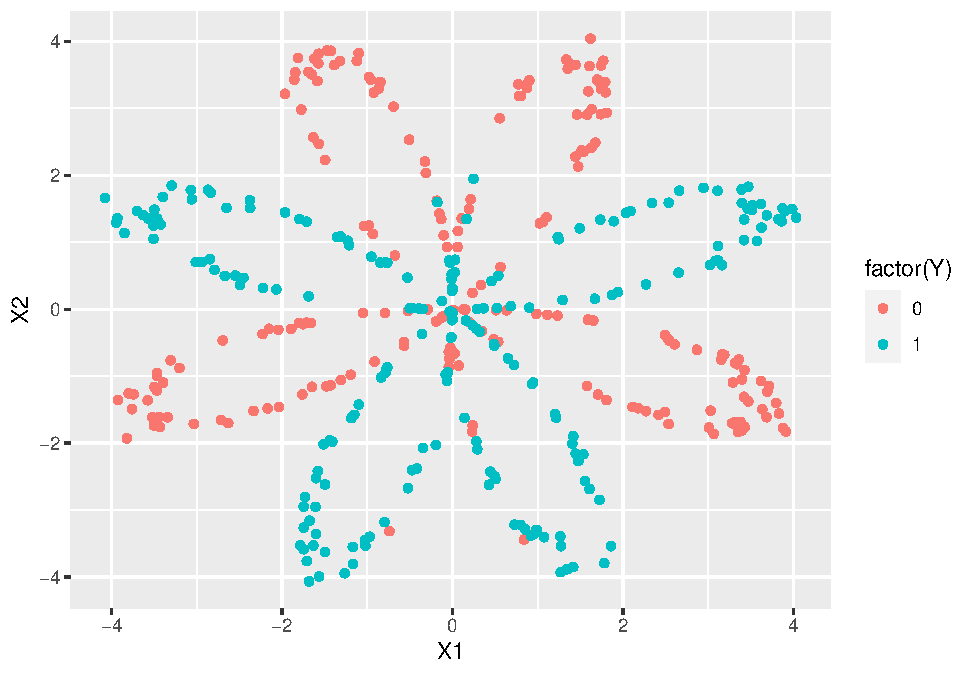
\includegraphics{BabyNeuralNet_files/unnamed-chunk-1-1.pdf}

\hypertarget{preprocessing}{%
\section{Preprocessing}\label{preprocessing}}

\hypertarget{traintest-split}{%
\subsection{Train/Test split}\label{traintest-split}}

\textbf{\emph{After I make this my own, change the data set and run a
70/30 split}}

\begin{Shaded}
\begin{Highlighting}[]
\FunctionTok{set.seed}\NormalTok{(}\DecValTok{69}\NormalTok{)}

\NormalTok{df }\OtherTok{\textless{}{-}}\NormalTok{ df[}\FunctionTok{sample}\NormalTok{(}\FunctionTok{nrow}\NormalTok{(df)), ]  }\CommentTok{\#shuffle the data}
\FunctionTok{head}\NormalTok{(df)}
\end{Highlighting}
\end{Shaded}

\begin{verbatim}
##             X1          X2 Y
## 209 -1.6819006 -4.06622254 1
## 347 -2.8676777  1.78432368 1
## 386  0.1415769 -1.62418643 1
## 112  1.2314394 -0.09522700 0
## 104  1.1126080 -0.08436755 0
## 111  0.6345588 -0.01693373 0
\end{verbatim}

\begin{Shaded}
\begin{Highlighting}[]
\NormalTok{train\_test\_split }\OtherTok{\textless{}{-}} \FloatTok{0.7} \SpecialCharTok{*} \FunctionTok{nrow}\NormalTok{(df)  }\CommentTok{\#70\% of data into our train set and the remaining 30\% in our test set}

\NormalTok{train }\OtherTok{\textless{}{-}}\NormalTok{ df[}\DecValTok{1}\SpecialCharTok{:}\NormalTok{train\_test\_split,]  }\CommentTok{\#extracting first (shuffled) 70\% of rows into a dataset}
\FunctionTok{head}\NormalTok{(train)}
\end{Highlighting}
\end{Shaded}

\begin{verbatim}
##             X1          X2 Y
## 209 -1.6819006 -4.06622254 1
## 347 -2.8676777  1.78432368 1
## 386  0.1415769 -1.62418643 1
## 112  1.2314394 -0.09522700 0
## 104  1.1126080 -0.08436755 0
## 111  0.6345588 -0.01693373 0
\end{verbatim}

\begin{Shaded}
\begin{Highlighting}[]
\NormalTok{test }\OtherTok{\textless{}{-}}\NormalTok{ df[(train\_test\_split}\SpecialCharTok{+}\DecValTok{1}\NormalTok{)}\SpecialCharTok{:} \FunctionTok{nrow}\NormalTok{(df),] }\CommentTok{\#extracting remaining (shuffled) 20\% of rows into test datset}
\FunctionTok{head}\NormalTok{(test)}
\end{Highlighting}
\end{Shaded}

\begin{verbatim}
##             X1         X2 Y
## 375  0.9197000 -3.3827722 1
## 182 -0.1536376  1.4300506 0
## 174 -1.6894987  3.5457345 0
## 86  -2.6943985 -0.4667928 0
## 346 -1.2120203  0.9559181 1
## 76  -3.4675772 -1.2134685 0
\end{verbatim}

\hypertarget{assess-for-class-imbalance}{%
\subsection{Assess for Class
Imbalance}\label{assess-for-class-imbalance}}

\begin{Shaded}
\begin{Highlighting}[]
\CommentTok{\#plots and numeric proportions of classes to assess for severe imbalance}
\CommentTok{\#for train:}
\NormalTok{trainplot }\OtherTok{\textless{}{-}} \FunctionTok{ggplot}\NormalTok{(train, }\FunctionTok{aes}\NormalTok{(}\AttributeTok{x =}\NormalTok{ Y, }\AttributeTok{fill =} \FunctionTok{factor}\NormalTok{(Y))) }\SpecialCharTok{+}
  \FunctionTok{geom\_bar}\NormalTok{(}\FunctionTok{aes}\NormalTok{(}\AttributeTok{y =}\NormalTok{ (..count..)}\SpecialCharTok{/}\FunctionTok{sum}\NormalTok{(..count..)))}

\NormalTok{fortrain }\OtherTok{\textless{}{-}} \FunctionTok{round}\NormalTok{(}\FunctionTok{prop.table}\NormalTok{(}\FunctionTok{table}\NormalTok{(train}\SpecialCharTok{$}\NormalTok{Y)), }\DecValTok{3}\NormalTok{) }

\CommentTok{\#for test:}
\NormalTok{testplot }\OtherTok{\textless{}{-}} \FunctionTok{ggplot}\NormalTok{(test, }\FunctionTok{aes}\NormalTok{(}\AttributeTok{x =}\NormalTok{ Y, }\AttributeTok{fill =} \FunctionTok{factor}\NormalTok{(Y))) }\SpecialCharTok{+}
  \FunctionTok{geom\_bar}\NormalTok{(}\FunctionTok{aes}\NormalTok{(}\AttributeTok{y =}\NormalTok{ (..count..)}\SpecialCharTok{/}\FunctionTok{sum}\NormalTok{(..count..)))}

\NormalTok{fortest }\OtherTok{\textless{}{-}} \FunctionTok{round}\NormalTok{(}\FunctionTok{prop.table}\NormalTok{(}\FunctionTok{table}\NormalTok{(test}\SpecialCharTok{$}\NormalTok{Y)), }\DecValTok{3}\NormalTok{)}

\FunctionTok{grid.arrange}\NormalTok{(trainplot }\SpecialCharTok{+} \FunctionTok{labs}\NormalTok{(}\AttributeTok{title =} \StringTok{"Training data"}\NormalTok{, }\AttributeTok{fill=}\StringTok{"classification"}\NormalTok{, }\AttributeTok{y =} \StringTok{"Proportion of Each Class"}\NormalTok{), testplot  }\SpecialCharTok{+} \FunctionTok{labs}\NormalTok{(}\AttributeTok{title =} \StringTok{"Test data"}\NormalTok{, }\AttributeTok{fill=}\StringTok{"classification"}\NormalTok{, }\AttributeTok{y =} \StringTok{"Proportion of Each Class"}\NormalTok{), }\AttributeTok{ncol =} \DecValTok{2}\NormalTok{)}
\end{Highlighting}
\end{Shaded}

\begin{verbatim}
## Warning: The dot-dot notation (`..count..`) was deprecated in ggplot2 3.4.0.
## i Please use `after_stat(count)` instead.
\end{verbatim}

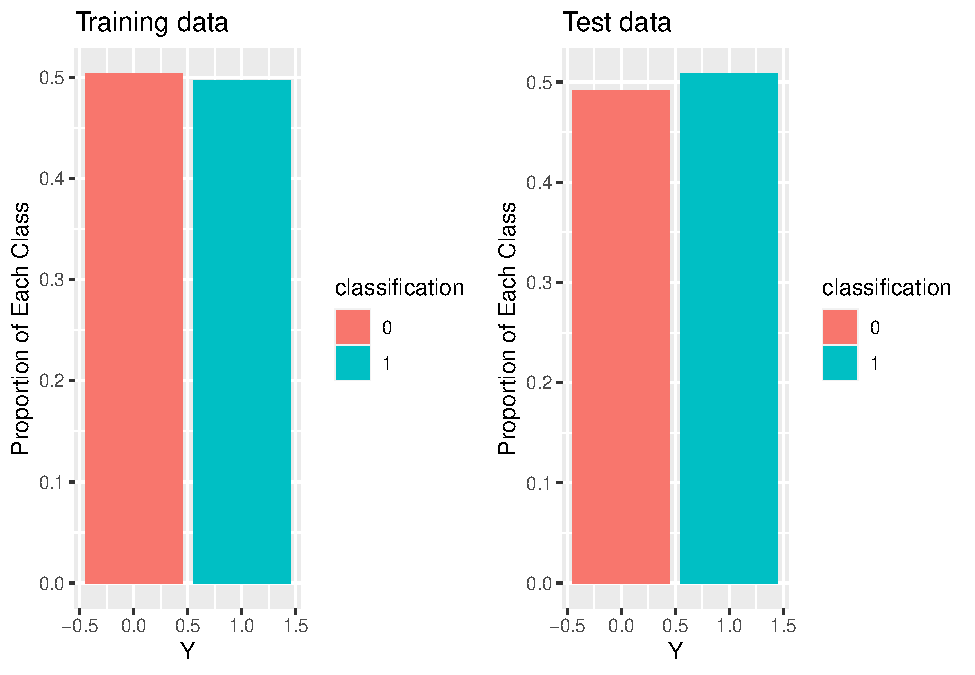
\includegraphics{BabyNeuralNet_files/unnamed-chunk-3-1.pdf}

The relevant proportions of each class for the training data is 0.504,
0.496.\\
The relevant proportions of each class for the test data is 0.492,
0.508.

\hypertarget{standardize}{%
\subsection{Standardize}\label{standardize}}

We normalize the data to ensure that our activation functions take both
positive and negative values. If we have features that are all positive
or all negative, the learning process will zig-zag toward extrema very
wildly and make learning harder. By standardizing, we not only avoid
this but also ensure that the distributions of our weights and bias are
the same (and therefore they will learn at nearly the same rate), making
for faster convergence.

\begin{Shaded}
\begin{Highlighting}[]
\CommentTok{\#standardizing the data}
\DocumentationTok{\#\#note that we are standardizing the input values, not the output (Y) values}

\NormalTok{train\_x }\OtherTok{\textless{}{-}} \FunctionTok{scale}\NormalTok{(train[, }\FunctionTok{c}\NormalTok{(}\DecValTok{1}\SpecialCharTok{:}\DecValTok{2}\NormalTok{)])   }\CommentTok{\#standardize all rows in the second two columns (X1 and X2)}
\NormalTok{train\_y }\OtherTok{\textless{}{-}}\NormalTok{ train}\SpecialCharTok{$}\NormalTok{Y}
\FunctionTok{dim}\NormalTok{(train\_y) }\OtherTok{\textless{}{-}} \FunctionTok{c}\NormalTok{(}\FunctionTok{length}\NormalTok{(train\_y), }\DecValTok{1}\NormalTok{) }\CommentTok{\# add extra dimension to vector}

\NormalTok{test\_x }\OtherTok{\textless{}{-}} \FunctionTok{scale}\NormalTok{(test[, }\FunctionTok{c}\NormalTok{(}\DecValTok{1}\SpecialCharTok{:}\DecValTok{2}\NormalTok{)])}
\NormalTok{test\_y }\OtherTok{\textless{}{-}}\NormalTok{ test}\SpecialCharTok{$}\NormalTok{Y}
\FunctionTok{dim}\NormalTok{(test\_y) }\OtherTok{\textless{}{-}} \FunctionTok{c}\NormalTok{(}\FunctionTok{length}\NormalTok{(test\_y), }\DecValTok{1}\NormalTok{) }\CommentTok{\# add extra dimension to vector}
\end{Highlighting}
\end{Shaded}

\hypertarget{convert-to-matrices}{%
\subsection{Convert to Matrices}\label{convert-to-matrices}}

Converting to matrices speeds up the calculation.

\begin{Shaded}
\begin{Highlighting}[]
\CommentTok{\#converting dataframes to matrices, and taking the transpose, for matrix multiplications}
\NormalTok{train\_x }\OtherTok{\textless{}{-}} \FunctionTok{as.matrix}\NormalTok{(train\_x, }\AttributeTok{byrow=}\ConstantTok{TRUE}\NormalTok{)}
\NormalTok{train\_x }\OtherTok{\textless{}{-}} \FunctionTok{t}\NormalTok{(train\_x)                     }\CommentTok{\#transpose}
\NormalTok{train\_y }\OtherTok{\textless{}{-}} \FunctionTok{as.matrix}\NormalTok{(train\_y, }\AttributeTok{byrow=}\ConstantTok{TRUE}\NormalTok{)}
\NormalTok{train\_y }\OtherTok{\textless{}{-}} \FunctionTok{t}\NormalTok{(train\_y)}

\NormalTok{test\_x }\OtherTok{\textless{}{-}} \FunctionTok{as.matrix}\NormalTok{(test\_x, }\AttributeTok{byrow=}\ConstantTok{TRUE}\NormalTok{)}
\NormalTok{test\_x }\OtherTok{\textless{}{-}} \FunctionTok{t}\NormalTok{(test\_x)}
\NormalTok{test\_y }\OtherTok{\textless{}{-}} \FunctionTok{as.matrix}\NormalTok{(test\_y, }\AttributeTok{byrow=}\ConstantTok{TRUE}\NormalTok{)}
\NormalTok{test\_y }\OtherTok{\textless{}{-}} \FunctionTok{t}\NormalTok{(test\_y)}


\CommentTok{\#shapes of matrices (to confirm with HTML reference page)}
\FunctionTok{dim}\NormalTok{(train\_x)}
\end{Highlighting}
\end{Shaded}

\begin{verbatim}
## [1]   2 280
\end{verbatim}

\begin{Shaded}
\begin{Highlighting}[]
\FunctionTok{dim}\NormalTok{(train\_y)}
\end{Highlighting}
\end{Shaded}

\begin{verbatim}
## [1]   1 280
\end{verbatim}

\begin{Shaded}
\begin{Highlighting}[]
\FunctionTok{dim}\NormalTok{(test\_x)}
\end{Highlighting}
\end{Shaded}

\begin{verbatim}
## [1]   2 120
\end{verbatim}

\begin{Shaded}
\begin{Highlighting}[]
\FunctionTok{dim}\NormalTok{(test\_y)}
\end{Highlighting}
\end{Shaded}

\begin{verbatim}
## [1]   1 120
\end{verbatim}

\hypertarget{building-the-network}{%
\section{Building the Network}\label{building-the-network}}

\hypertarget{layer-sizes}{%
\subsection{Layer Sizes}\label{layer-sizes}}

(Write about layer sizes here)

\hypertarget{function-in-r}{%
\subsubsection{Function in R:}\label{function-in-r}}

(Explain this function in more detail)

\begin{Shaded}
\begin{Highlighting}[]
\NormalTok{LayerSize }\OtherTok{\textless{}{-}} \ControlFlowTok{function}\NormalTok{(x, y, hidden, }\AttributeTok{train=}\ConstantTok{TRUE}\NormalTok{) \{}
\NormalTok{  n\_x }\OtherTok{\textless{}{-}} \FunctionTok{dim}\NormalTok{(x)[}\DecValTok{1}\NormalTok{]  }\CommentTok{\#returns the value of 2 based on the dimensions (train\_x is (2*280))}
\NormalTok{  n\_h }\OtherTok{\textless{}{-}}\NormalTok{ hidden     }\CommentTok{\# number of neurons in the hidden layer}
\NormalTok{  n\_y }\OtherTok{\textless{}{-}} \FunctionTok{dim}\NormalTok{(y)[}\DecValTok{1}\NormalTok{]  }\CommentTok{\#returns the value of 1 (train\_y is (1*280))}
  
\NormalTok{  size }\OtherTok{\textless{}{-}} \FunctionTok{list}\NormalTok{(}\StringTok{"Input layer size"} \OtherTok{=}\NormalTok{ n\_x,}
               \StringTok{"Hidden layer size"} \OtherTok{=}\NormalTok{ n\_h,}
               \StringTok{"Output layer size"} \OtherTok{=}\NormalTok{ n\_y)}
  
  \FunctionTok{return}\NormalTok{(size)}
\NormalTok{\}}
\NormalTok{layer\_size }\OtherTok{\textless{}{-}} \FunctionTok{LayerSize}\NormalTok{(train\_x, train\_y, }\AttributeTok{hidden =} \DecValTok{4}\NormalTok{)}
\NormalTok{layer\_size }\CommentTok{\#returns a list of each layers\textquotesingle{} sizes}
\end{Highlighting}
\end{Shaded}

\begin{verbatim}
## $`Input layer size`
## [1] 2
## 
## $`Hidden layer size`
## [1] 4
## 
## $`Output layer size`
## [1] 1
\end{verbatim}

\begin{itemize}
\tightlist
\item
  The input layer has 2 neurons.
\item
  The hidden layer has 4 neurons.
\item
  The output layer has 1 neurons.
\end{itemize}

\hypertarget{initialize-parameters}{%
\subsection{Initialize parameters}\label{initialize-parameters}}

We will select our starting parameters from a uniform distribution
\(Unif(0,1)\).\\
Because this network has three layers, we will have two sets of
parameters (a matrix of weights and a matrix of biases for both the
input layer and for the hidden layer).

\begin{itemize}
\tightlist
\item
  The shape of the weight matrix for the input layer is
  \((N_{hidden},N_{input})\)
\item
  The shape of the bias matrix for the input layer is \((N_{hidden},1)\)
\item
  The shape of the weight matrix for the hidden layer is
  \((N_{output},N_{hidden})\)
\item
  The shape of the bias matrix for the hidden layer is
  \((N_{output},1)\)
\end{itemize}

\hypertarget{function-in-r-1}{%
\subsubsection{Function in R:}\label{function-in-r-1}}

(Explain this function in more detail)

\begin{Shaded}
\begin{Highlighting}[]
\NormalTok{initializeParameters }\OtherTok{\textless{}{-}} \ControlFlowTok{function}\NormalTok{(X, layer\_sizes)\{}

\NormalTok{  m }\OtherTok{\textless{}{-}} \FunctionTok{dim}\NormalTok{(}\FunctionTok{data.matrix}\NormalTok{(X))[}\DecValTok{1}\NormalTok{]}
  
\NormalTok{  n\_x }\OtherTok{\textless{}{-}}\NormalTok{ layer\_sizes[[}\DecValTok{1}\NormalTok{]]}
\NormalTok{  n\_h }\OtherTok{\textless{}{-}}\NormalTok{ layer\_sizes[[}\DecValTok{2}\NormalTok{]]}
\NormalTok{  n\_y }\OtherTok{\textless{}{-}}\NormalTok{ layer\_sizes[[}\DecValTok{3}\NormalTok{]]}
  
\NormalTok{  W1 }\OtherTok{\textless{}{-}} \FunctionTok{matrix}\NormalTok{(}\FunctionTok{runif}\NormalTok{(n\_h }\SpecialCharTok{*}\NormalTok{ n\_x), }\AttributeTok{nrow =}\NormalTok{ n\_h, }\AttributeTok{ncol =}\NormalTok{ n\_x, }\AttributeTok{byrow =} \ConstantTok{TRUE}\NormalTok{) }\SpecialCharTok{*} \FloatTok{0.01}
\NormalTok{  b1 }\OtherTok{\textless{}{-}} \FunctionTok{matrix}\NormalTok{(}\FunctionTok{rep}\NormalTok{(}\DecValTok{0}\NormalTok{, n\_h), }\AttributeTok{nrow =}\NormalTok{ n\_h)}
\NormalTok{  W2 }\OtherTok{\textless{}{-}} \FunctionTok{matrix}\NormalTok{(}\FunctionTok{runif}\NormalTok{(n\_y }\SpecialCharTok{*}\NormalTok{ n\_h), }\AttributeTok{nrow =}\NormalTok{ n\_y, }\AttributeTok{ncol =}\NormalTok{ n\_h, }\AttributeTok{byrow =} \ConstantTok{TRUE}\NormalTok{) }\SpecialCharTok{*} \FloatTok{0.01}
\NormalTok{  b2 }\OtherTok{\textless{}{-}} \FunctionTok{matrix}\NormalTok{(}\FunctionTok{rep}\NormalTok{(}\DecValTok{0}\NormalTok{, n\_y), }\AttributeTok{nrow =}\NormalTok{ n\_y)}
  
\NormalTok{  params }\OtherTok{\textless{}{-}} \FunctionTok{list}\NormalTok{(}\StringTok{"Initial weights layer 1 (W1)"} \OtherTok{=}\NormalTok{ W1,}
                 \StringTok{"Initial biases layer 1 (b1)"} \OtherTok{=}\NormalTok{ b1, }
                 \StringTok{"Initial weights hidden layer (W2)"} \OtherTok{=}\NormalTok{ W2,}
                 \StringTok{"Initial biases hidden layer (b2)"} \OtherTok{=}\NormalTok{ b2)}
  
  \FunctionTok{return}\NormalTok{ (params)}
\NormalTok{\}}

\NormalTok{init\_params }\OtherTok{\textless{}{-}} \FunctionTok{initializeParameters}\NormalTok{(train\_x, layer\_size)}
\FunctionTok{lapply}\NormalTok{(init\_params, }\ControlFlowTok{function}\NormalTok{(x) }\FunctionTok{dim}\NormalTok{(x))}
\end{Highlighting}
\end{Shaded}

\begin{verbatim}
## $`Initial weights layer 1 (W1)`
## [1] 4 2
## 
## $`Initial biases layer 1 (b1)`
## [1] 4 1
## 
## $`Initial weights hidden layer (W2)`
## [1] 1 4
## 
## $`Initial biases hidden layer (b2)`
## [1] 1 1
\end{verbatim}

\begin{itemize}
\tightlist
\item
  The shape of the weight matrix for the input layer is (4, 2)
\item
  The shape of the bias matrix for the input layer is (4, 1)
\item
  The shape of the weight matrix for the hidden layer is (1, 4)
\item
  The shape of the bias matrix for the hidden layer is (1, 1)
\end{itemize}

\hypertarget{activation-functions}{%
\subsection{Activation Functions}\label{activation-functions}}

(Write about activation functions and discuss their differences.)

\begin{Shaded}
\begin{Highlighting}[]
\CommentTok{\#creating and plotting the sigmoid function}
\NormalTok{sigmoid }\OtherTok{\textless{}{-}} \ControlFlowTok{function}\NormalTok{(x)\{}
  \FunctionTok{return}\NormalTok{(}\DecValTok{1} \SpecialCharTok{/}\NormalTok{ (}\DecValTok{1} \SpecialCharTok{+} \FunctionTok{exp}\NormalTok{(}\SpecialCharTok{{-}}\NormalTok{x)))}
\NormalTok{\}}

\NormalTok{relu }\OtherTok{\textless{}{-}} \ControlFlowTok{function}\NormalTok{(x)\{}
  \FunctionTok{ifelse}\NormalTok{ (x}\SpecialCharTok{\textless{}}\DecValTok{0}\NormalTok{,}\DecValTok{0}\NormalTok{,x) }
\NormalTok{\}}

\NormalTok{lrelu }\OtherTok{\textless{}{-}} \ControlFlowTok{function}\NormalTok{(x)\{}
  \FunctionTok{ifelse}\NormalTok{ (x}\SpecialCharTok{\textless{}}\DecValTok{0}\NormalTok{,}\FloatTok{0.1}\SpecialCharTok{*}\NormalTok{x,x) }
\NormalTok{\}}

\NormalTok{f }\OtherTok{\textless{}{-}} \FunctionTok{seq}\NormalTok{(}\SpecialCharTok{{-}}\DecValTok{8}\NormalTok{,}\DecValTok{8}\NormalTok{, }\AttributeTok{length=}\DecValTok{1000}\NormalTok{)}

\FunctionTok{plot}\NormalTok{(f,}\FunctionTok{sigmoid}\NormalTok{(f), }\AttributeTok{main=}\StringTok{"Sigmoid"}\NormalTok{, }\AttributeTok{xlab =} \StringTok{" "}\NormalTok{, }\AttributeTok{ylab =} \StringTok{" "}\NormalTok{)}
\FunctionTok{plot}\NormalTok{(f,}\FunctionTok{tanh}\NormalTok{(f), }\AttributeTok{main=}\StringTok{"Hyperbolic Tangent"}\NormalTok{, }\AttributeTok{xlab =} \StringTok{" "}\NormalTok{, }\AttributeTok{ylab =} \StringTok{" "}\NormalTok{)}
\FunctionTok{plot}\NormalTok{(f,}\FunctionTok{relu}\NormalTok{(f), }\AttributeTok{main=}\StringTok{"ReLU"}\NormalTok{, }\AttributeTok{xlab =} \StringTok{" "}\NormalTok{, }\AttributeTok{ylab =} \StringTok{" "}\NormalTok{)}
\FunctionTok{plot}\NormalTok{(f,}\FunctionTok{lrelu}\NormalTok{(f), }\AttributeTok{main=}\StringTok{"Leaky ReLU"}\NormalTok{, }\AttributeTok{xlab =} \StringTok{" "}\NormalTok{, }\AttributeTok{ylab =} \StringTok{" "}\NormalTok{)}
\end{Highlighting}
\end{Shaded}

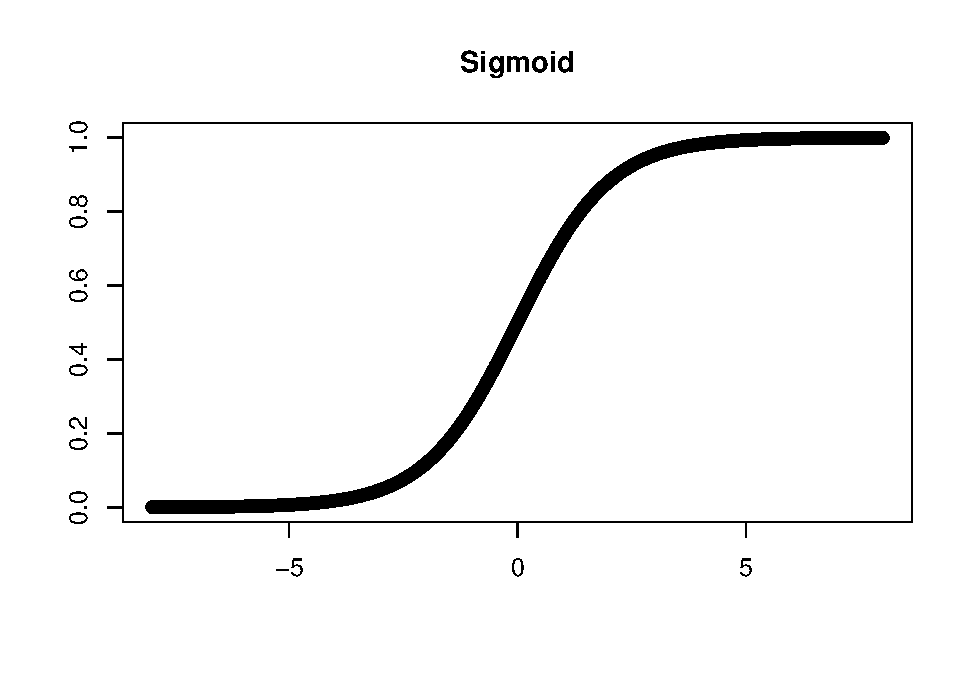
\includegraphics[width=0.5\linewidth]{BabyNeuralNet_files/figures-side-1}
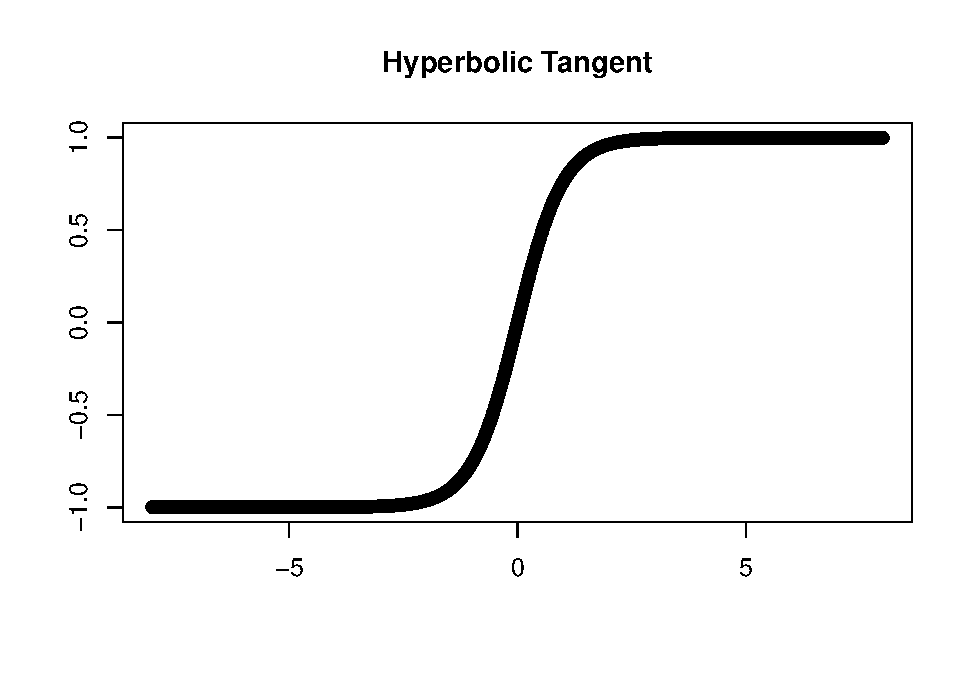
\includegraphics[width=0.5\linewidth]{BabyNeuralNet_files/figures-side-2}
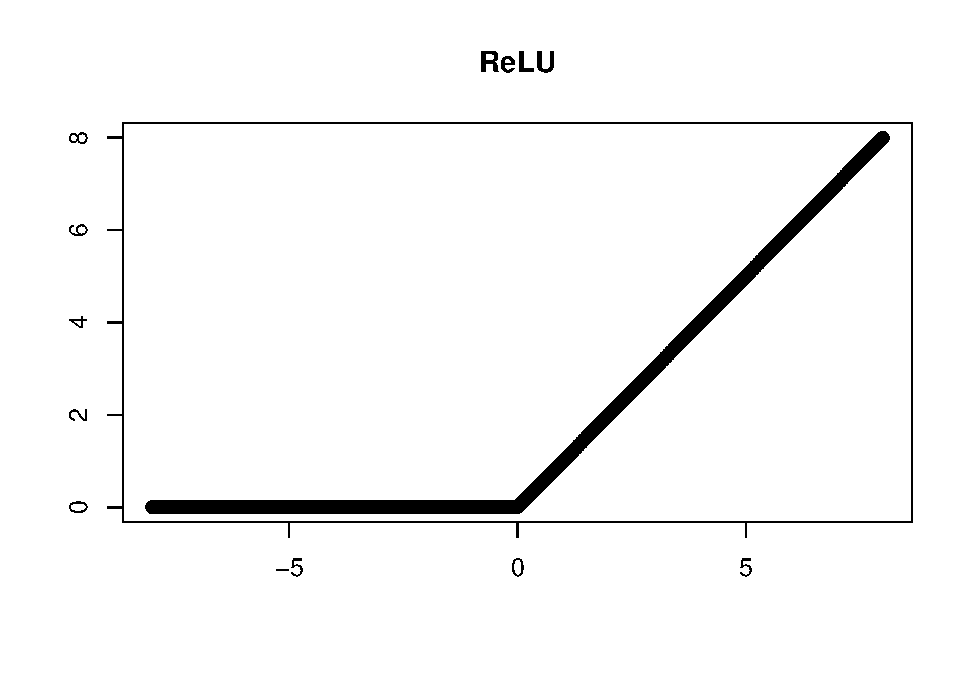
\includegraphics[width=0.5\linewidth]{BabyNeuralNet_files/figures-side-3}
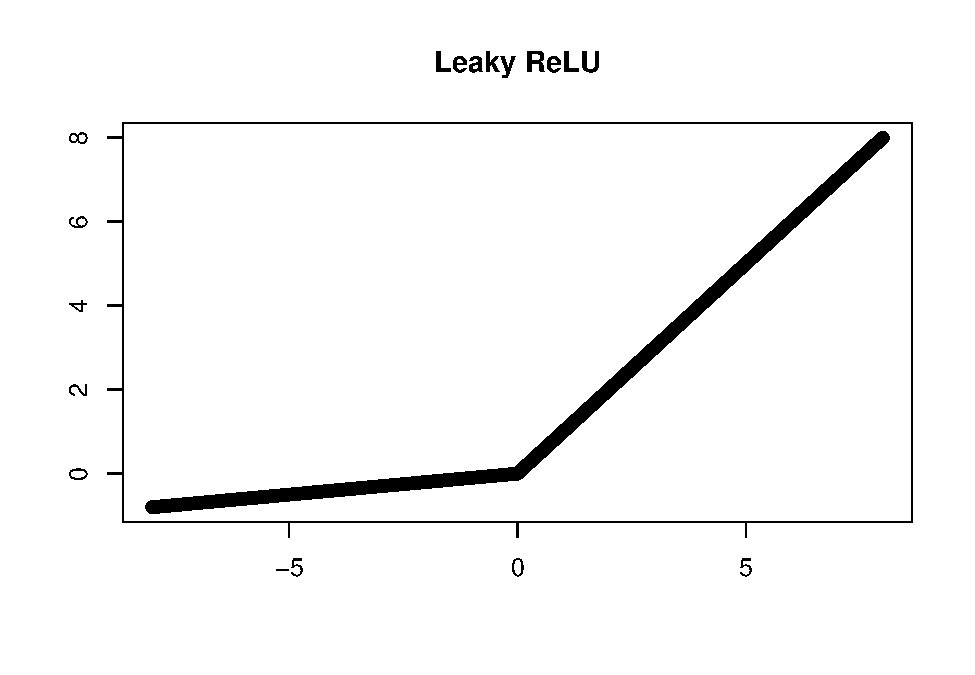
\includegraphics[width=0.5\linewidth]{BabyNeuralNet_files/figures-side-4}

\hypertarget{forward-propagation}{%
\subsection{Forward Propagation}\label{forward-propagation}}

(write about this step)

\hypertarget{function-in-r-2}{%
\subsubsection{Function in R:}\label{function-in-r-2}}

(refine the details of this function)

matrix multiplication dimensions: \texttt{W1\ \%*\%\ X} dimensions:
\texttt{(4,2)} x \texttt{(2,320)} = \texttt{(4,320)}
\texttt{W2\ \%*\%\ A1} dimensions: \texttt{(1,4)} x \texttt{(4,320)} =
\texttt{(1,320)}

The \texttt{forward} function uses the input training data, the weights
and biases (starting with the initial ones calculated above), and the
size of the layers to propagate forward through the network.\\
After calling the relevant parameters, the function first repeats the
biases to be able to add that bias to each component of the preceding
multiplication. The function multiplies the matrix of input training
values by the matrix of weights to pass through the first layer of the
network, adds the bias to each value of the resulting matrix, and passes
that through the activation function. It then multiplies the resulting
matrix by the matrix of weights in the hidden layer, finalizing by
passing it through another activation function.

\begin{Shaded}
\begin{Highlighting}[]
\NormalTok{forward }\OtherTok{\textless{}{-}} \ControlFlowTok{function}\NormalTok{(X, params, layer\_sizes)\{}
\CommentTok{\#function of the input matrix (X), the list of parameters, and the list of layer sizes}
  
\NormalTok{  m }\OtherTok{\textless{}{-}} \FunctionTok{dim}\NormalTok{(X)[}\DecValTok{2}\NormalTok{]  }\CommentTok{\#second dimension of shape x (280)}
\NormalTok{  n\_h }\OtherTok{\textless{}{-}}\NormalTok{ layer\_sizes[[}\DecValTok{2}\NormalTok{]]}
\NormalTok{  n\_y }\OtherTok{\textless{}{-}}\NormalTok{ layer\_sizes[[}\DecValTok{3}\NormalTok{]]}
  
\NormalTok{  W1 }\OtherTok{\textless{}{-}}\NormalTok{ params[[}\DecValTok{1}\NormalTok{]]}
\NormalTok{  b1 }\OtherTok{\textless{}{-}}\NormalTok{ params[[}\DecValTok{2}\NormalTok{]]}
\NormalTok{  W2 }\OtherTok{\textless{}{-}}\NormalTok{ params[[}\DecValTok{3}\NormalTok{]]}
\NormalTok{  b2 }\OtherTok{\textless{}{-}}\NormalTok{ params[[}\DecValTok{4}\NormalTok{]]}
  
\NormalTok{  b1\_new }\OtherTok{\textless{}{-}} \FunctionTok{matrix}\NormalTok{(}\FunctionTok{rep}\NormalTok{(b1, m), }\AttributeTok{nrow =}\NormalTok{ n\_h)  }\CommentTok{\#repeat b1 to be able to add the bias to each component of the matrix                                               multiplication step (weight*input)}
\NormalTok{  b2\_new }\OtherTok{\textless{}{-}} \FunctionTok{matrix}\NormalTok{(}\FunctionTok{rep}\NormalTok{(b2, m), }\AttributeTok{nrow =}\NormalTok{ n\_y)  }\CommentTok{\#repeat b1 to be able to add the bias to each component of the matrix                                               multiplication step (weight*hidden)}
  
\NormalTok{  Z1 }\OtherTok{\textless{}{-}}\NormalTok{ W1 }\SpecialCharTok{\%*\%}\NormalTok{ X }\SpecialCharTok{+}\NormalTok{ b1\_new  }\CommentTok{\#(input to hidden) matrix multiplication of weight and input matrix}
\NormalTok{  A1 }\OtherTok{\textless{}{-}} \FunctionTok{sigmoid}\NormalTok{(Z1) }\CommentTok{\#activation function for the previous line}
\NormalTok{  Z2 }\OtherTok{\textless{}{-}}\NormalTok{ W2 }\SpecialCharTok{\%*\%}\NormalTok{ A1 }\SpecialCharTok{+}\NormalTok{ b2\_new }\CommentTok{\#(hidden to output) matrix multiplication of weights and hidden layer matrix}
\NormalTok{  A2 }\OtherTok{\textless{}{-}} \FunctionTok{sigmoid}\NormalTok{(Z2) }\CommentTok{\#activation function for the previous line}

  
\NormalTok{  cache }\OtherTok{\textless{}{-}} \FunctionTok{list}\NormalTok{(}\StringTok{"Z1"} \OtherTok{=}\NormalTok{ Z1,}
                \StringTok{"A1"} \OtherTok{=}\NormalTok{ A1, }
                \StringTok{"Z2"} \OtherTok{=}\NormalTok{ Z2,}
                \StringTok{"A2"} \OtherTok{=}\NormalTok{ A2)}
  
  \FunctionTok{return}\NormalTok{ (cache)}
\NormalTok{\}}

\CommentTok{\#matrix multiplications explained:}
\CommentTok{\# W1 \%*\% X dimensions: (4,2)*(2,320) = (4,320)}
\CommentTok{\# W2 \%*\% A1 dimensions: (1,4)*(4,320) = (1,320)}
\CommentTok{\#biases are repeated so to be added to each component of the respective matrix}

\NormalTok{fwd\_prop }\OtherTok{\textless{}{-}} \FunctionTok{forward}\NormalTok{(train\_x, init\_params, layer\_size)}
\FunctionTok{lapply}\NormalTok{(fwd\_prop, }\ControlFlowTok{function}\NormalTok{(x) }\FunctionTok{dim}\NormalTok{(x))}
\end{Highlighting}
\end{Shaded}

\begin{verbatim}
## $Z1
## [1]   4 280
## 
## $A1
## [1]   4 280
## 
## $Z2
## [1]   1 280
## 
## $A2
## [1]   1 280
\end{verbatim}

\begin{itemize}
\tightlist
\item
  Output matrix from the input layer: (4, 280)
\item
  Activation function: (4, 280)
\item
  Output matrix from the hidden layer: (1, 280)
\item
  Activation function (end result per iteration ): (1, 280)
\end{itemize}

All four calculations are stored to be used in the backpropagation
algorithm, but first the final calculation is used to compute cost.

\hypertarget{computing-cost}{%
\subsection{Computing Cost}\label{computing-cost}}

(Change this completely to utilize the correct loss function)

uses the Mean Squared Error loss function to compare true values with
predicted output

\[
C = \frac{1}{n} \sum_{i=1}^N (a^{(L)}_i - y_i)
\] Where \(a^{(L)}_i\) is the outcome of a single iteration of forward
propagation and \(y_i\) is the true observation to compare it to.

\hypertarget{function-in-r-3}{%
\subsubsection{Function in R}\label{function-in-r-3}}

(Change this to reflect the correct loss function)\\
(Explain this function in more detail)

\begin{Shaded}
\begin{Highlighting}[]
\NormalTok{costComp }\OtherTok{\textless{}{-}} \ControlFlowTok{function}\NormalTok{(X, y, cache) \{}
\NormalTok{  m }\OtherTok{\textless{}{-}} \FunctionTok{dim}\NormalTok{(X)[}\DecValTok{2}\NormalTok{]}
\NormalTok{  A2 }\OtherTok{\textless{}{-}}\NormalTok{ cache[[}\DecValTok{4}\NormalTok{]]  }\CommentTok{\#y{-}hat}
\NormalTok{  logprobs }\OtherTok{\textless{}{-}}\NormalTok{ (}\FunctionTok{log}\NormalTok{(A2) }\SpecialCharTok{*}\NormalTok{ y) }\SpecialCharTok{+}\NormalTok{ (}\FunctionTok{log}\NormalTok{(}\DecValTok{1}\SpecialCharTok{{-}}\NormalTok{A2) }\SpecialCharTok{*}\NormalTok{ (}\DecValTok{1}\SpecialCharTok{{-}}\NormalTok{y))}
\NormalTok{  cost }\OtherTok{\textless{}{-}} \SpecialCharTok{{-}}\FunctionTok{sum}\NormalTok{(logprobs}\SpecialCharTok{/}\NormalTok{m)}
  \FunctionTok{return}\NormalTok{ (cost)}
\NormalTok{\}}
\NormalTok{cost }\OtherTok{\textless{}{-}} \FunctionTok{costComp}\NormalTok{(train\_x, train\_y, fwd\_prop)}
\NormalTok{cost}
\end{Highlighting}
\end{Shaded}

\begin{verbatim}
## [1] 0.6932143
\end{verbatim}

\hypertarget{backpropagation}{%
\subsection{Backpropagation}\label{backpropagation}}

\textbf{Backpropagation} is the algorithm that computes the gradient for
high-dimensional derivatives for the process of \textbf{gradient
descent}, which helps us reduce the cost function. For a standard neural
network, it is composed of the partial derivatives of the cost function
with respect to each weight in each layer of the network, and each bias
in each layer of the network.

\[
\nabla{C} =
\begin{bmatrix}
\frac{\partial{C}}{\partial{w_1^{(1)}}} & \frac{\partial{C}}{\partial{w_2^{(1)}}} & \cdots & 
\frac{\partial{C}}{\partial{w_i^{(1)}}} \\
\frac{\partial{C}}{\partial{b_1^{(1)}}} & \frac{\partial{C}}{\partial{b_2^{(1)}}} & \cdots & 
\frac{\partial{C}}{\partial{b_i^{(1)}}} \\
\vdots & \vdots & \ddots & \vdots \\
\frac{\partial{C}}{\partial{w_1^{(l)}}} & \frac{\partial{C}}{\partial{w_2^{(l)}}} & \cdots & 
\frac{\partial{C}}{\partial{w_i^{(l)}}} \\
\frac{\partial{C}}{\partial{b_1^{(l)}}} & \frac{\partial{C}}{\partial{b_2^{(l)}}} & \cdots & 
\frac{\partial{C}}{\partial{b_i^{(l)}}} \\
\end{bmatrix}
\] Here, the superscript \(^{(l)}\) denotes the layer of the network and
the subscript \(_i\) denotes a specific parameter within that specific
layer. Since we have two layers, \(^{(2)}\) indicates the hidden layer
and \(^{(1)}\) the input layer.

\hypertarget{theoretical-formulation}{%
\subsubsection{Theoretical Formulation}\label{theoretical-formulation}}

The backpropagation algorithm is catered to a specific loss function. In
this example, the loss function is defined above as \emph{Mean Squared
Error}. This function takes the difference between the output from the
network and the specified desired output for each observation. To
understand how each parameter that makes up the output must be adjusted,
the algorithm must differentiate every part of it. This is done by use
of the chain rule in calculus. Ultimately, two parameter
differentiations must be computed for each observation in each layer - a
\emph{weight} and a \emph{bias}, as illustrated in the matrix above.

The chain rule is applied when tracing the lineage of influence on the
network's output. In tracing the architecture of the network backwards
(or ``back propagating''), the output is found to be influenced by:

\begin{itemize}
\tightlist
\item
  an activation function in between the hidden layer and the output,
  which is influenced by the resulting computation of the hidden layer
  \emph{weight}, \emph{bias}, and
\item
  an activation function from the previous layer, which is which is
  influenced by the resulting computation of the previous layer
  \emph{weight}, \emph{bias}, and activation of earlier layers.
\end{itemize}

Because our network only has an input and hidden layer, this
``previous'' layer is the input layer, and the ``activation of earlier
layers'' is our input x-value.

\hypertarget{partial-derivatives-with-respect-to-weight}{%
\paragraph{Partial derivatives with respect to
weight}\label{partial-derivatives-with-respect-to-weight}}

The amount we must adjust the weight in the \emph{hidden} layer is
represented by: \$\$ \begin{eqnarray}
\frac{\partial{C}}{\partial{w_i^{(2)}}}    &=&  \dfrac{\partial{z_i^{(2)}}}{\partial{w_i^{(2)}}}
     \dfrac{\partial{a_i^{(2)}}}{\partial{z_i^{(2)}}}
     \dfrac{\partial{C}}{\partial{a_i^{(2)}}} \\
     
 &=& a_i^{(1)} \sigma'(z_i^{(2)}) 2(a_i^{(2)}-y_i) \\
\end{eqnarray} \$\$

Where \(a_n^{(1)}\) is the activation for each observation in the first
(input) layer, \(\sigma'(z_i^{(2)})\) is the derivative of the sigmoid
activation function with respect to each observation in the second
(hidden) layer, \(a_i^{(2)}\) is the activation for each observation in
the hidden layer, and \(y_i\) is the vector of actual training values
this network hopes to achieve.

The amount we must adjust the weight in the \emph{input} layer is
represented by: \$\$ \begin{eqnarray}
\frac{\partial{C}}{\partial{w_i^{(1)}}}    &=& \dfrac{\partial{z_i^{(1)}}}{\partial{w_i^{(1)}}} \dfrac{\partial{a_i^{(1)}}}{\partial{z_i^{(1)}}}  \dfrac{\partial{z_i^{(2)}}}{\partial{a_i^{(1)}}}
     \dfrac{\partial{a_i^{(2)}}}{\partial{z_i^{(2)}}}
     \dfrac{\partial{C}}{\partial{a_i^{(2)}}} \\
     
&=& x_i \sigma'(z_i^{(1)}) w_i^{(2)} \sigma'(z_i^{(2)}) 2(a_i^{(2)}-y_i) \\

\end{eqnarray} \$\$ where \(x_i\) is the input from our training data,
\(\sigma'(z_i^{(1)})\) is the derivative of the sigmoid activation
function with respect to each observation in the input layer,
\(w_i^{(2)}\) is the vector of weights in the hidden layer, and all else
is the same as is in the previous equation.

\hypertarget{partial-derivatives-with-respect-to-bias}{%
\paragraph{Partial derivatives with respect to
bias}\label{partial-derivatives-with-respect-to-bias}}

The amount we must adjust the bias in the \emph{hidden} layer is
represented by: \[
\frac{\partial{C}}{\partial{b_i^{(2)}}}  =  \dfrac{\partial{z_i^{(2)}}}{\partial{b_i^{(2)}}}
     \dfrac{\partial{a_i^{(2)}}}{\partial{z_i^{(2)}}}
     \dfrac{\partial{C}}{\partial{a_i^{(2)}}} \\
\]

Because the bias is a constant, that is
\(\dfrac{\partial{z_i^{(l)}}}{\partial{b_i^{(l)}}} = 1\), our chain-rule
formula simplifies to the following: \[
\frac{\partial{C}}{\partial{b_i^{(2)}}} = 1 \cdot \sigma'(z_i^{(2)}) 2(a_i^{(2)}-y_i) \\
\]

The amount we must adjust the bias in the \emph{input} layer is
represented by: \$\$ \begin{eqnarray}
\frac{\partial{C}}{\partial{b_i^{(1)}}}    &=& \dfrac{\partial{z_i^{(1)}}}{\partial{b_i^{(1)}}} \dfrac{\partial{a_i^{(1)}}}{\partial{z_i^{(1)}}}  \dfrac{\partial{z_i^{(2)}}}{\partial{a_i^{(1)}}}
     \dfrac{\partial{a_i^{(2)}}}{\partial{z_i^{(2)}}}
     \dfrac{\partial{C}}{\partial{a_i^{(2)}}} \\
     
&=& 1 \cdot \sigma'(z_i^{(1)}) w_i^{(2)} \sigma'(z_i^{(2)}) 2(a_i^{(2)}-y_i) \\

\end{eqnarray} \$\$

\hypertarget{function-in-r-4}{%
\subsubsection{Function in R:}\label{function-in-r-4}}

Below is the function that computes backpropagation for the \emph{Mean
Square Error} loss function.

\begin{itemize}
\tightlist
\item
  \texttt{dW1}contains the necessary adjustment needed to the weights in
  the input layer \(\frac{\partial{C}}{\partial{w_i^{(1)}}}\)
\item
  \texttt{dW2}contains the necessary adjustment needed to the weights in
  the hidden layer \(\frac{\partial{C}}{\partial{w_i^{(2)}}}\)
\item
  \texttt{dB1}contains contains the necessary adjustment needed to the
  biases in the input layer \(\frac{\partial{C}}{\partial{b_i^{(1)}}}\)
\item
  \texttt{dB2}contains contains the necessary adjustment needed to the
  biases in the hidden layer \(\frac{\partial{C}}{\partial{b_i^{(2)}}}\)
\end{itemize}

\begin{Shaded}
\begin{Highlighting}[]
\NormalTok{dxsigmoid }\OtherTok{\textless{}{-}} \ControlFlowTok{function}\NormalTok{(x) \{}
\NormalTok{  (}\DecValTok{1}\SpecialCharTok{/}\NormalTok{(}\DecValTok{1}\SpecialCharTok{+}\FunctionTok{exp}\NormalTok{(}\SpecialCharTok{{-}}\NormalTok{x))) }\SpecialCharTok{*}\NormalTok{ (}\DecValTok{1} \SpecialCharTok{{-}}\NormalTok{ (}\DecValTok{1}\SpecialCharTok{/}\NormalTok{(}\DecValTok{1}\SpecialCharTok{+}\FunctionTok{exp}\NormalTok{(}\SpecialCharTok{{-}}\NormalTok{x))))}
\NormalTok{\}}

\CommentTok{\#not correct derivative below; used for testing stuff}
\CommentTok{\#dxsigmoid \textless{}{-} function(x) \{}
\CommentTok{\#  x * (1.0 {-} x)}
\CommentTok{\#\}}
\DocumentationTok{\#\#\#\#}

\NormalTok{backp }\OtherTok{\textless{}{-}} \ControlFlowTok{function}\NormalTok{(x, y, cache, params,layer\_sizes)\{}

\NormalTok{  A2 }\OtherTok{\textless{}{-}}\NormalTok{ cache[[}\DecValTok{4}\NormalTok{]]}
\NormalTok{  A1 }\OtherTok{\textless{}{-}}\NormalTok{ cache[[}\DecValTok{2}\NormalTok{]]}
\NormalTok{  Z2 }\OtherTok{\textless{}{-}}\NormalTok{ cache[[}\DecValTok{3}\NormalTok{]]}
\NormalTok{  W2 }\OtherTok{\textless{}{-}}\NormalTok{ params[[}\DecValTok{3}\NormalTok{]]}
\NormalTok{  Z1 }\OtherTok{\textless{}{-}}\NormalTok{ cache[[}\DecValTok{1}\NormalTok{]]}
  
\NormalTok{    m }\OtherTok{\textless{}{-}} \FunctionTok{dim}\NormalTok{(x)[}\DecValTok{2}\NormalTok{]}
  
\NormalTok{  n\_x }\OtherTok{\textless{}{-}}\NormalTok{ layer\_sizes[[}\DecValTok{1}\NormalTok{]]}
\NormalTok{  n\_h }\OtherTok{\textless{}{-}}\NormalTok{ layer\_sizes[[}\DecValTok{2}\NormalTok{]]}
\NormalTok{  n\_y }\OtherTok{\textless{}{-}}\NormalTok{ layer\_sizes[[}\DecValTok{3}\NormalTok{]]}
  
\NormalTok{  dW2 }\OtherTok{\textless{}{-}}\NormalTok{ A1 }\SpecialCharTok{\%*\%} \FunctionTok{t}\NormalTok{(}\FunctionTok{dxsigmoid}\NormalTok{(Z2) }\SpecialCharTok{*} \DecValTok{2}\SpecialCharTok{*}\NormalTok{(A2}\SpecialCharTok{{-}}\NormalTok{y)) }\CommentTok{\#CRUCIAL INFO {-} look at matrix multipliers}
  
\NormalTok{  dW1 }\OtherTok{\textless{}{-}} \FunctionTok{t}\NormalTok{(W2) }\SpecialCharTok{\%*\%}\NormalTok{ (}\FunctionTok{dxsigmoid}\NormalTok{(Z2) }\SpecialCharTok{*} \DecValTok{2}\SpecialCharTok{*}\NormalTok{(A2}\SpecialCharTok{{-}}\NormalTok{y))}
\NormalTok{  dW1 }\OtherTok{\textless{}{-}}\NormalTok{ dW1}\SpecialCharTok{*}\FunctionTok{dxsigmoid}\NormalTok{(Z1)}
\NormalTok{  dW1 }\OtherTok{\textless{}{-}}\NormalTok{ dW1 }\SpecialCharTok{\%*\%} \FunctionTok{t}\NormalTok{(x)}
  
\NormalTok{  dB2 }\OtherTok{\textless{}{-}} \FunctionTok{matrix}\NormalTok{(}\FunctionTok{dxsigmoid}\NormalTok{(Z2) }\SpecialCharTok{\%*\%} \FunctionTok{t}\NormalTok{(}\DecValTok{2}\SpecialCharTok{*}\NormalTok{(A2}\SpecialCharTok{{-}}\NormalTok{y)), }\AttributeTok{nrow =}\NormalTok{ n\_y)}
\CommentTok{\#  dB2 \textless{}{-} matrix(rep(dB2, m), nrow = n\_y) }
  
\NormalTok{  dB1 }\OtherTok{\textless{}{-}} \FunctionTok{matrix}\NormalTok{((W2 }\SpecialCharTok{\%*\%} \FunctionTok{dxsigmoid}\NormalTok{(Z1) }\SpecialCharTok{\%*\%} \FunctionTok{t}\NormalTok{(}\FunctionTok{dxsigmoid}\NormalTok{(Z2) }\SpecialCharTok{*} \DecValTok{2}\SpecialCharTok{*}\NormalTok{(A2}\SpecialCharTok{{-}}\NormalTok{y))) , }\AttributeTok{ncol =}\NormalTok{ n\_h)}
\CommentTok{\#  dB1 \textless{}{-} matrix(rep(dB1, m), nrow = n\_h)}
  
\NormalTok{    gradient }\OtherTok{\textless{}{-}} \FunctionTok{list}\NormalTok{(}\StringTok{"dW1"} \OtherTok{=}\NormalTok{ dW1,}
                     \StringTok{"dW2"} \OtherTok{=}\NormalTok{ dW2,}
                     \StringTok{"dB1"} \OtherTok{=}\NormalTok{ dB1,}
                     \StringTok{"dB2"} \OtherTok{=}\NormalTok{ dB2)}
  
  \FunctionTok{return}\NormalTok{(gradient)}
    
\NormalTok{\}}

\NormalTok{back }\OtherTok{\textless{}{-}} \FunctionTok{backp}\NormalTok{(train\_x, train\_y, fwd\_prop, init\_params,layer\_size)}
\NormalTok{back}
\end{Highlighting}
\end{Shaded}

\begin{verbatim}
## $dW1
##               X1         X2
## [1,] 0.007784623 0.01220243
## [2,] 0.012377554 0.01940226
## [3,] 0.012336751 0.01933869
## [4,] 0.019159197 0.03003465
## 
## $dW2
##           [,1]
## [1,] 0.4873600
## [2,] 0.4856782
## [3,] 0.4760061
## [4,] 0.4908793
## 
## $dB1
##             [,1]        [,2]        [,3]        [,4]
## [1,] 0.005843082 0.005843082 0.005843082 0.005843082
## 
## $dB2
##           [,1]
## [1,] 0.9366386
\end{verbatim}

\begin{itemize}
\tightlist
\item
  The shape of the weight matrix for the input layer is (4, 2)
\item
  The shape of the bias matrix for the input layer is (4, 1)
\item
  The shape of the weight matrix for the hidden layer is (1, 4)
\item
  The shape of the bias matrix for the hidden layer is (1, 1)
\end{itemize}

\hypertarget{updating-parameters}{%
\subsection{Updating parameters}\label{updating-parameters}}

Parameters are updated by applying the gradient fro the previous step to
the respective weights and biases. Since the aim is to reduce the cost,
we \emph{subtract} the gradient terms. Additionally, a ``step size'' is
multiplied to the gradient terms to moderate how fast the machine
learns: too large a step and the machine can bounce in and out of the
desired minimum; too small and it will be very computationally costly to
reach the desired point.

\begin{Shaded}
\begin{Highlighting}[]
\NormalTok{updateParameters }\OtherTok{\textless{}{-}} \ControlFlowTok{function}\NormalTok{(gradient, params, stepsize)\{}
  
\NormalTok{  W1 }\OtherTok{\textless{}{-}}\NormalTok{ params[[}\DecValTok{1}\NormalTok{]]}
\NormalTok{  b1 }\OtherTok{\textless{}{-}}\NormalTok{ params[[}\DecValTok{2}\NormalTok{]]}
\NormalTok{  W2 }\OtherTok{\textless{}{-}}\NormalTok{ params[[}\DecValTok{3}\NormalTok{]]}
\NormalTok{  b2 }\OtherTok{\textless{}{-}}\NormalTok{ params[[}\DecValTok{4}\NormalTok{]]}
  
\NormalTok{  dW1 }\OtherTok{\textless{}{-}}\NormalTok{ gradient[[}\DecValTok{1}\NormalTok{]]}
\NormalTok{  db1 }\OtherTok{\textless{}{-}}\NormalTok{ gradient[[}\DecValTok{2}\NormalTok{]]}
\NormalTok{  dW2 }\OtherTok{\textless{}{-}}\NormalTok{ gradient[[}\DecValTok{3}\NormalTok{]]}
\NormalTok{  db2 }\OtherTok{\textless{}{-}}\NormalTok{ gradient[[}\DecValTok{4}\NormalTok{]]}
  
\NormalTok{  W1 }\OtherTok{\textless{}{-}}\NormalTok{ W1 }\SpecialCharTok{{-}}\NormalTok{ stepsize }\SpecialCharTok{*}\NormalTok{ dW1}
\NormalTok{  b1 }\OtherTok{\textless{}{-}}\NormalTok{ b1 }\SpecialCharTok{{-}}\NormalTok{ stepsize }\SpecialCharTok{*}\NormalTok{ db1}
\NormalTok{  W2 }\OtherTok{\textless{}{-}}\NormalTok{ W2 }\SpecialCharTok{{-}}\NormalTok{ stepsize }\SpecialCharTok{*}\NormalTok{ dW2}
\NormalTok{  b2 }\OtherTok{\textless{}{-}}\NormalTok{ b2 }\SpecialCharTok{{-}}\NormalTok{ stepsize }\SpecialCharTok{*}\NormalTok{ db2}
  
\NormalTok{  updated\_params }\OtherTok{\textless{}{-}} \FunctionTok{list}\NormalTok{(}\StringTok{"W1"} \OtherTok{=}\NormalTok{ W1,}
                         \StringTok{"b1"} \OtherTok{=}\NormalTok{ b1,}
                         \StringTok{"W2"} \OtherTok{=}\NormalTok{ W2,}
                         \StringTok{"b2"} \OtherTok{=}\NormalTok{ b2)}
  
  \FunctionTok{return}\NormalTok{ (updated\_params)}
\NormalTok{\}}

\NormalTok{update\_params }\OtherTok{\textless{}{-}} \FunctionTok{updateParameters}\NormalTok{(back, init\_params, }\AttributeTok{stepsize =} \FloatTok{0.01}\NormalTok{)}
\CommentTok{\#lapply(update\_params, function(x) dim(x))}
\end{Highlighting}
\end{Shaded}

Initial matrix for the weights in layer 1: \[\begin{bmatrix}
0.00252167382510379&0.00425880226772279 \\
0.0038607051433064&0.00288630024762824 \\
0.00270326758502051&0.000644203233532608 \\
0.00862992925802246&0.00144658315228298 \\
\end{bmatrix}\]

updated matrix for the weights in layer 1: \[\begin{bmatrix}
0.00244382759798631&0.00413677798849759 \\
0.00373692960083072&0.00269227765399693 \\
0.00257990007837287&0.000450816337493054 \\
0.00843833729175307&0.00114623668063622 \\
\end{bmatrix}\]

If we subtract the two and multiply by 100 to reverse the step size, we
can see that the results are exactly identical to the results for the
weights in the first layer from the backpropagation step - so we're
still on track!

\begin{Shaded}
\begin{Highlighting}[]
\NormalTok{(init\_params[[}\DecValTok{1}\NormalTok{]] }\SpecialCharTok{{-}}\NormalTok{ update\_params[[}\DecValTok{1}\NormalTok{]])}\SpecialCharTok{*}\DecValTok{100}
\end{Highlighting}
\end{Shaded}

\begin{verbatim}
##               X1         X2
## [1,] 0.007784623 0.01220243
## [2,] 0.012377554 0.01940226
## [3,] 0.012336751 0.01933869
## [4,] 0.019159197 0.03003465
\end{verbatim}

\begin{Shaded}
\begin{Highlighting}[]
\NormalTok{back[[}\DecValTok{1}\NormalTok{]]}
\end{Highlighting}
\end{Shaded}

\begin{verbatim}
##               X1         X2
## [1,] 0.007784623 0.01220243
## [2,] 0.012377554 0.01940226
## [3,] 0.012336751 0.01933869
## [4,] 0.019159197 0.03003465
\end{verbatim}

\hypertarget{training-the-model}{%
\section{Training the Model}\label{training-the-model}}

\hypertarget{conclusion}{%
\section{Conclusion}\label{conclusion}}

\hypertarget{references}{%
\subsection{References}\label{references}}

\href{https://rviews.rstudio.com/2020/07/20/shallow-neural-net-from-scratch-using-r-part-1/}{R
Views page part 1}\\
\href{https://rviews.rstudio.com/2020/07/24/building-a-neural-net-from-scratch-using-r-part-2/}{R
Views page part 2}\\
\href{https://www.3blue1brown.com/lessons/backpropagation-calculus}{3Blue1Brown
lesson}\\
Nielsen (2015) Rumelhart, Hinton, and Williams (1986)

\hypertarget{refs}{}
\begin{CSLReferences}{1}{0}
\leavevmode\vadjust pre{\hypertarget{ref-nielsen}{}}%
Nielsen, Michael A. 2015. \emph{Neural Networks and Deep Learning}.
Determination press.

\leavevmode\vadjust pre{\hypertarget{ref-Rumelhart1986LearningRB}{}}%
Rumelhart, David E., Geoffrey E. Hinton, and Ronald J. Williams. 1986.
{``Learning Representations by Back-Propagating Errors.''} \emph{Nature}
323: 533--36.

\end{CSLReferences}

